% Options for packages loaded elsewhere
\PassOptionsToPackage{unicode}{hyperref}
\PassOptionsToPackage{hyphens}{url}
%
\documentclass[
]{book}
\usepackage{amsmath,amssymb}
\usepackage{lmodern}
\usepackage{iftex}
\ifPDFTeX
  \usepackage[T1]{fontenc}
  \usepackage[utf8]{inputenc}
  \usepackage{textcomp} % provide euro and other symbols
\else % if luatex or xetex
  \usepackage{unicode-math}
  \defaultfontfeatures{Scale=MatchLowercase}
  \defaultfontfeatures[\rmfamily]{Ligatures=TeX,Scale=1}
\fi
% Use upquote if available, for straight quotes in verbatim environments
\IfFileExists{upquote.sty}{\usepackage{upquote}}{}
\IfFileExists{microtype.sty}{% use microtype if available
  \usepackage[]{microtype}
  \UseMicrotypeSet[protrusion]{basicmath} % disable protrusion for tt fonts
}{}
\makeatletter
\@ifundefined{KOMAClassName}{% if non-KOMA class
  \IfFileExists{parskip.sty}{%
    \usepackage{parskip}
  }{% else
    \setlength{\parindent}{0pt}
    \setlength{\parskip}{6pt plus 2pt minus 1pt}}
}{% if KOMA class
  \KOMAoptions{parskip=half}}
\makeatother
\usepackage{xcolor}
\usepackage{longtable,booktabs,array}
\usepackage{calc} % for calculating minipage widths
% Correct order of tables after \paragraph or \subparagraph
\usepackage{etoolbox}
\makeatletter
\patchcmd\longtable{\par}{\if@noskipsec\mbox{}\fi\par}{}{}
\makeatother
% Allow footnotes in longtable head/foot
\IfFileExists{footnotehyper.sty}{\usepackage{footnotehyper}}{\usepackage{footnote}}
\makesavenoteenv{longtable}
\usepackage{graphicx}
\makeatletter
\def\maxwidth{\ifdim\Gin@nat@width>\linewidth\linewidth\else\Gin@nat@width\fi}
\def\maxheight{\ifdim\Gin@nat@height>\textheight\textheight\else\Gin@nat@height\fi}
\makeatother
% Scale images if necessary, so that they will not overflow the page
% margins by default, and it is still possible to overwrite the defaults
% using explicit options in \includegraphics[width, height, ...]{}
\setkeys{Gin}{width=\maxwidth,height=\maxheight,keepaspectratio}
% Set default figure placement to htbp
\makeatletter
\def\fps@figure{htbp}
\makeatother
\setlength{\emergencystretch}{3em} % prevent overfull lines
\providecommand{\tightlist}{%
  \setlength{\itemsep}{0pt}\setlength{\parskip}{0pt}}
\setcounter{secnumdepth}{5}
\ifLuaTeX
\usepackage[bidi=basic]{babel}
\else
\usepackage[bidi=default]{babel}
\fi
\babelprovide[main,import]{brazilian}
% get rid of language-specific shorthands (see #6817):
\let\LanguageShortHands\languageshorthands
\def\languageshorthands#1{}
\usepackage{booktabs}
\ifLuaTeX
  \usepackage{selnolig}  % disable illegal ligatures
\fi
\usepackage[]{natbib}
\bibliographystyle{plainnat}
\IfFileExists{bookmark.sty}{\usepackage{bookmark}}{\usepackage{hyperref}}
\IfFileExists{xurl.sty}{\usepackage{xurl}}{} % add URL line breaks if available
\urlstyle{same} % disable monospaced font for URLs
\hypersetup{
  pdftitle={Template Book - Disciplina},
  pdfauthor={Daniel Claudino},
  pdflang={pt-BR},
  hidelinks,
  pdfcreator={LaTeX via pandoc}}

\title{Template Book - Disciplina}
\author{Daniel Claudino}
\date{2022-10-16}

\begin{document}
\maketitle

{
\setcounter{tocdepth}{1}
\tableofcontents
}
\hypertarget{apresentauxe7uxe3o-da-disciplina}{%
\chapter{Apresentação da Disciplina}\label{apresentauxe7uxe3o-da-disciplina}}

NOME DA DISCIPLINA

\begin{figure}

{\centering 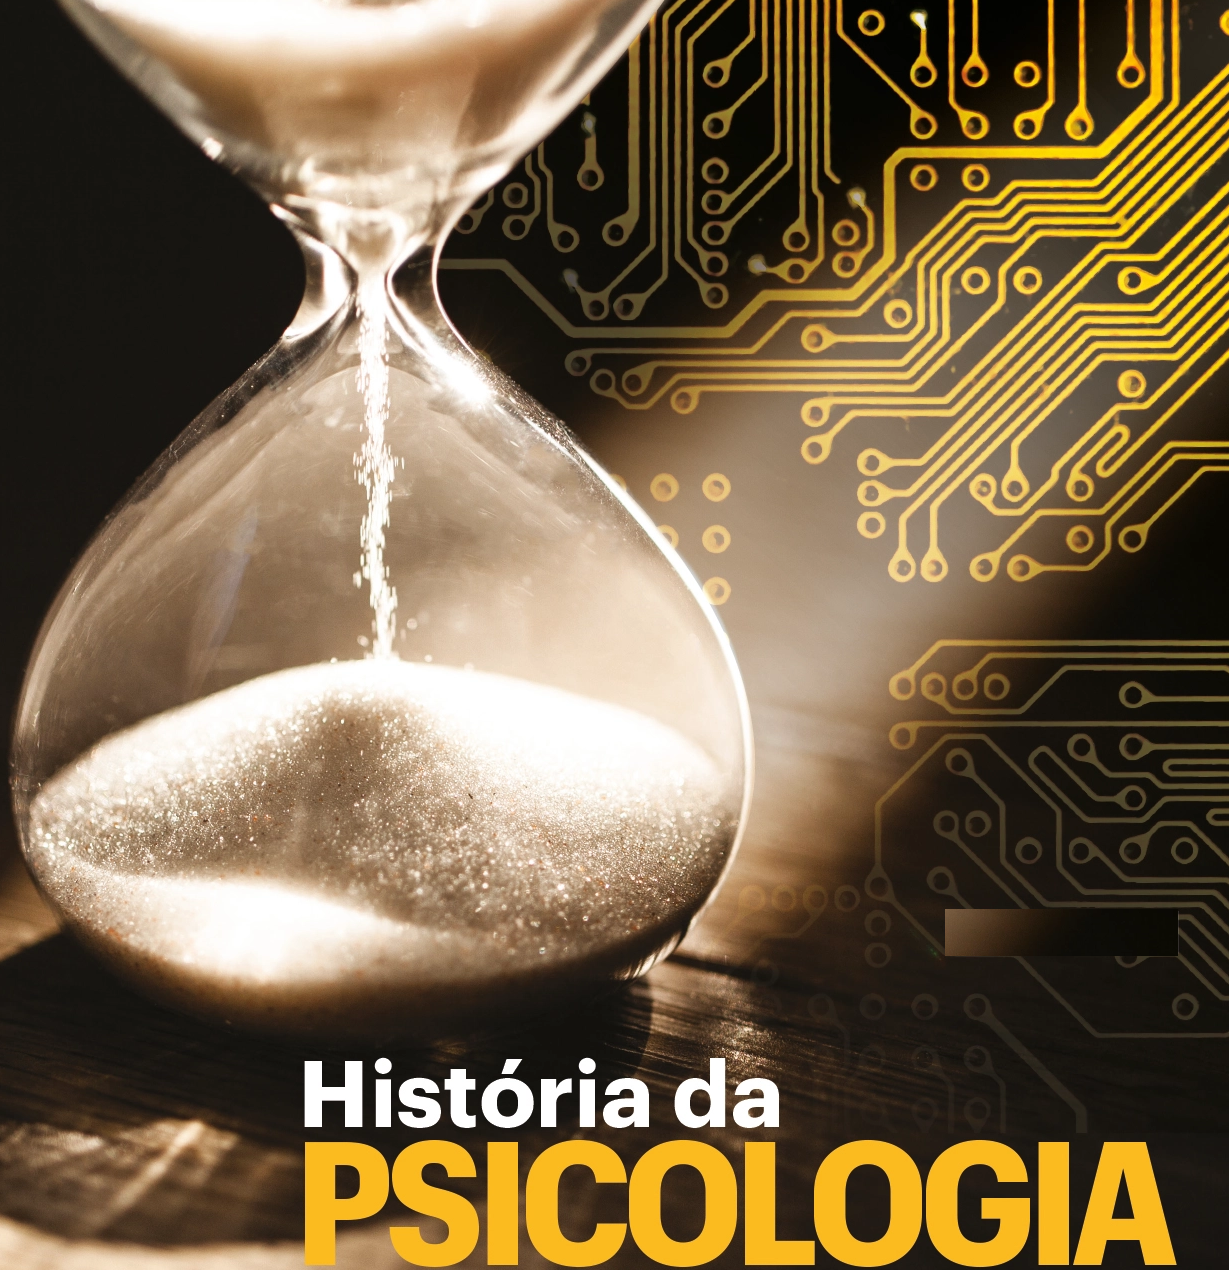
\includegraphics[width=0.5\linewidth]{figuras/capa-livro-historia-da-psicologia-schultz} 

}

\caption{Capa}\label{fig:unnamed-chunk-1}
\end{figure}

\begin{itemize}
\tightlist
\item
  Neste material, estão contidos:

  \begin{itemize}
  \tightlist
  \item
    Minhas notas de aula;
  \item
    Notas de Aula de outros colegas disponibilizados para a turma
  \item
    Resumos de capítulos de livros;
  \item
    Resumos de apresentações(slides) da disciplina;
  \item
    Resumos de outros colegas de sala disponibilizados para a turma;
  \item
    Minhas apresentações(slides);

    \begin{itemize}
    \tightlist
    \item
      Audience Q\&A (Permite que o público das apresentação envie perguntas para o apresntador)
    \item
      Live Polls (Permite que o público das apresntações realize votações sobre os temas apresentados)
    \item
      Quiz (Permite que o público das apresentações participe de competições integrando-se e assimilando melhor os temas apresentados)
    \end{itemize}
  \item
    Exercício elaborados pelos professores, respondidos ou não em sala;
  \item
    Questionários elaborados por mim antes das provas;
  \item
    Formulários de pesquisa (Google Forms) elaborados por mim para atendimento de necessidades dos dos meus colegas de sala, dos professores ou da disciplina;
  \item
    Coletas de dados realizadas para atendimento de necessidades dos dos meus colegas de sala, dos professores ou da disciplina;
  \item
    Planilhas elaboradas por mim elaboradas por mim para atendimento de necessidades dos dos meus colegas de sala, dos professores ou da disciplina;
  \item
    Filmes recomendados;
  \item
    Documentários recomendados;
  \item
    Jogos de aprendizado criados (Kahoots / Site principal: kahoot.com / Login do jogador: kahoot.it)
  \item
    Outros materiais elaborados e disponibilizados pelos professores e por mim.
  \end{itemize}
\end{itemize}

\hypertarget{professora}{%
\section{Professor(a)}\label{professora}}

\begin{itemize}
\tightlist
\item
  \textbf{Profª. Meª.} Nome-do-professor
\end{itemize}

\hypertarget{objetivos-da-disciplina}{%
\section{Objetivos da Disciplina}\label{objetivos-da-disciplina}}

\begin{quote}
Exemplo: A disciplina tem como objetivo proporcionar ao aluno os conhecimentos em relação à História da Psicologia através de suas raízes filosóficas e fisiológicas, bem como a compreensão das diversas escolas e suas epistemologias. Também pretende-se oportunizar o entendimento das diversas complexidades que envolvem as teorias psicológicas e seus respectivos autores.
\end{quote}

\hypertarget{ementa}{%
\section{Ementa}\label{ementa}}

\begin{quote}
Exemplo: A origem da Psicologia. Suas raízes filosóficas e fisiológicas, pensamento grego e teorias da idade média, moderna e renascentista. A Psicologia no seu desenvolvimento histórico. As grandes escolas da Psicologia. A Psicologia no contexto brasileiro atual.
\end{quote}

\hypertarget{conteuxfado-programuxe1tico}{%
\section{Conteúdo Programático}\label{conteuxfado-programuxe1tico}}

\begin{quote}
Exemplo: O primeiro módulo contemplará os estudo das raízes filosóficas e fisiológicas da Psicologia, trazendo o pensamento grego e suas implicações, as teorias vigentes na idade média, moderna e o renascimento e o desenvolvimento da Psicologia científica e experimental.
\end{quote}

\begin{quote}
No segundo módulo será abordado as grandes escolas da Psicologia: Estruturalismo, Funcionalismo, Behaviorismo, Gestalt, Psicanálise, Psicodrama, Fenomenologia e Existencialismo.
\end{quote}

\begin{quote}
Por fim, o terceiro módulo será composto pela análise histórica da Psicologia no
contexto brasileiro e a sua situação atual.
\end{quote}

\begin{quote}
4.1 Como tudo começou: As Raízes filosóficas e fisiológicas da Psicologia\\
4.1.1 Senso comum ou ciência? A Psicologia não é repetir mais do mesmo\\
4.1.2 Psicologia científica e não mística\\
4.1.3 A evolução do pensamento histórico da Psicologia\\
4.1.4 Raízes filosóficas Grega\\
4.1.5 Raízes filosóficas Romana\\
4.1.6 Raízes filosóficas da Idade Média\\
4.1.7 Raízes filosóficas do Renascimento\\
4.2 Vários caminhos a percorrer: As Grandes Escolas da Psicologia\\
4.2.1 Wundt para além da filosofia: o início da psicologia clínica\\
4.2.2 O Estruturalismo e Funcionalismo\\
4.2.3 O comportamento humano pode ser controlado: O Behaviorismo\\
4.2.4 Por uma Psicologia Plena: Rogers e o Humanismo\\
4.2.5 Um outro Eu que desconheço: A Psicanálise e o inconsciente\\
4.2.6 E depois de Freud, o que mudou?\\
4.3 Psicólogo para quê? A Psicologia atual e seus desafios\\
4.3.1 A Psicologia no Brasil
\end{quote}

\hypertarget{metodologia-diduxe1tica}{%
\section{Metodologia Didática}\label{metodologia-diduxe1tica}}

\begin{quote}
A disciplina será desenvolvida por meio da ação conjunta professor e aluno, exigindo, para tanto, participação ativa nas aulas. Os procedimentos de ensino e aprendizagem adotados serão aulas expositivas e discussão de temas propostos, leitura e apresentação de textos, estudo individual ou em grupo, seminários e realização de práticas interdisciplinares.
\end{quote}

\hypertarget{avaliauxe7uxe3o}{%
\section{Avaliação}\label{avaliauxe7uxe3o}}

\begin{longtable}[]{@{}lll@{}}
\toprule()
Avaliação & Data & Descrição \\
\midrule()
\endhead
1º Avaliação & dd/mm/aaaa & Prova (7 objetivas + 3 abertas) \\
1º Avaliação & dd/mm/aaaa & ``Mude minha opinião'' + TAE) \\
1º Avaliação & dd/mm/aaaa & Simulado + Avaliação Qualitativa \\
\bottomrule()
\end{longtable}

\hypertarget{trabalho-acaduxeamico-efetivo-tae-da-disciplina}{%
\section{Trabalho Acadêmico Efetivo (TAE) da disciplina}\label{trabalho-acaduxeamico-efetivo-tae-da-disciplina}}

\begin{longtable}[]{@{}
  >{\raggedright\arraybackslash}p{(\columnwidth - 4\tabcolsep) * \real{0.3333}}
  >{\raggedright\arraybackslash}p{(\columnwidth - 4\tabcolsep) * \real{0.3333}}
  >{\raggedright\arraybackslash}p{(\columnwidth - 4\tabcolsep) * \real{0.3333}}@{}}
\toprule()
\begin{minipage}[b]{\linewidth}\raggedright
TAE
\end{minipage} & \begin{minipage}[b]{\linewidth}\raggedright
Data
\end{minipage} & \begin{minipage}[b]{\linewidth}\raggedright
Descrição
\end{minipage} \\
\midrule()
\endhead
Único & dd/mm/aaaa & Criação do podcast. O discente deverá selecionar uma notícia apresentada na mídia e relacionar qual área ou como o psicólogo poderia auxiliar no assunto em questão.O TAE será com o grupo de jornal.Usar o aplicativo ANCHOR. - Até 2,0 pontos.\textbf{Data TAE:} 27 de outubro de 2022\textbf{Data Jornal:} 09 de novembro \\
\bottomrule()
\end{longtable}

\hypertarget{referuxeancias-bibliogruxe1ficas}{%
\section{Referências Bibliográficas}\label{referuxeancias-bibliogruxe1ficas}}

\hypertarget{referuxeancias-buxe1sicas}{%
\subsection{Referências Básicas}\label{referuxeancias-buxe1sicas}}

BOCK, A. M. B. (2008). Psicologias: uma introdução ao estudo de psicologia. 14ª Ed.
São Paulo: Saraiva, 2008.

HOTHERSALL, D. (2019). História da Psicologia (4th edição). Grupo A.

SCHULTZ, D. P., \& SCHULTZ, S. E. (2019). História da Psicologia Moderna -- Tradução da 11a
edição norte‐americana (4th edição). Cengage Learning Brasil.

\hypertarget{referuxeancias-complementares}{%
\subsection{Referências Complementares}\label{referuxeancias-complementares}}

Psicologia do Desenvolvimento. São Paulo, Contexto, 2014. {[}Livro Eletrônico{]} LIMA, C. F., \& PIMENTEL, C. E. (2017). Livro: Revisitando a Psicologia Social.

MISKOLCI, Richard. Teoria Queer: um aprendizado pelas diferenças. 2 ed.~Belo Horizonte: Autêntica, 2015. {[}Livro Eletrônico

PADILHA, S., NORONHA, A. P. P., \& ZANCHET, C. F. (2007). Instrumentos de avaliação psicológica: uso e parecer de psicólogos. Avaliação psicológica (páginas, 69-79). SCHULTZ, D. \& SCHULTZ, S. E. (2019). História da Psicologia moderna.

ZANELLI, J. C., BASTOS, A. V. B., \& RODRIGUES, A. C. A. ( 2014). Psicologia, Organizações e Trabalho no Brasil. (Orgs).

\hypertarget{controle-de-versuxe3o}{%
\section{Controle de Versão}\label{controle-de-versuxe3o}}

\begin{longtable}[]{@{}
  >{\raggedright\arraybackslash}p{(\columnwidth - 6\tabcolsep) * \real{0.2500}}
  >{\raggedright\arraybackslash}p{(\columnwidth - 6\tabcolsep) * \real{0.2500}}
  >{\raggedright\arraybackslash}p{(\columnwidth - 6\tabcolsep) * \real{0.2500}}
  >{\raggedright\arraybackslash}p{(\columnwidth - 6\tabcolsep) * \real{0.2500}}@{}}
\toprule()
\begin{minipage}[b]{\linewidth}\raggedright
Versão
\end{minipage} & \begin{minipage}[b]{\linewidth}\raggedright
Data / Hora
\end{minipage} & \begin{minipage}[b]{\linewidth}\raggedright
Colaborador
\end{minipage} & \begin{minipage}[b]{\linewidth}\raggedright
Descrição da Contribuição
\end{minipage} \\
\midrule()
\endhead
0.1 & 19/09/2022 11h00 & \href{https://wa.me/5583988853815}{Daniel Claudino} & Versão inicial do documento \\
0.2 & 05/10/2022 23h30 & \href{https://wa.me/5583988853815}{Daniel Claudino} & Acréscimo de informação no documento \\
\bottomrule()
\end{longtable}

\hypertarget{observauxe7uxe3o-importante}{%
\section{Observação Importante}\label{observauxe7uxe3o-importante}}

\textbf{NOTA}: Este material tem como finalidade auxiliar a fixação de assuntos estudados em sala de aula de acordo com o \textbf{plano de ensino desta disciplina}.

Ele \textbf{não deve ser} utilizado como \textbf{único material de estudo para a prova}, então:

\begin{enumerate}
\def\labelenumi{\arabic{enumi}.}
\tightlist
\item
  Consulte os \textbf{slides da professora} na plataforma FTM;\\
\item
  Faça \textbf{notas de aula} do que for tratado em sala de aula;\\
\item
  Consulte nossas \textbf{notas de aula};
\end{enumerate}

\begin{quote}
\textbf{Dúvidas}: Devem ser encaminhadas no grupo de whatsapp da disciplina.
\end{quote}

\hypertarget{resumo-das-apresentauxe7uxf5es-slides}{%
\chapter{Resumo das Apresentações (Slides)}\label{resumo-das-apresentauxe7uxf5es-slides}}

Neste capítulo estarão contidos meus resumos dos slides dos professores.

\hypertarget{slide-01---assuntos-da-aula}{%
\section{Slide 01 - ASSUNTOS DA AULA}\label{slide-01---assuntos-da-aula}}

\begin{longtable}[]{@{}ll@{}}
\toprule()
Data & Tópicos Abordados \\
\midrule()
\endhead
dd/mm/aaaa & - Tópico 1- Tópico 2- Tópico 3 \\
\bottomrule()
\end{longtable}

\hypertarget{seuxe7uxe3o-numerada-1}{%
\subsection{Seção Numerada 1}\label{seuxe7uxe3o-numerada-1}}

Para \citet{BOCK2001}, tornamo-nos pouco compreensíveis se não recorrermos a \ldots.

\hypertarget{seuxe7uxe3o-nuxe3o-numerada-1}{%
\subsection*{Seção não Numerada 1}\label{seuxe7uxe3o-nuxe3o-numerada-1}}
\addcontentsline{toc}{subsection}{Seção não Numerada 1}

Para \citet{BOCK2001}, tornamo-nos pouco compreensíveis se não recorrermos a \ldots.

\hypertarget{seuxe7uxe3o-nuxe3o-numerada-2}{%
\subsection*{Seção não Numerada 2}\label{seuxe7uxe3o-nuxe3o-numerada-2}}
\addcontentsline{toc}{subsection}{Seção não Numerada 2}

Para \citet{BOCK2001}, tornamo-nos pouco compreensíveis se não recorrermos a \ldots.

\hypertarget{seuxe7uxe3o-numerada-2}{%
\subsection{Seção Numerada 2}\label{seuxe7uxe3o-numerada-2}}

Para \citet{BOCK2001}, tornamo-nos pouco compreensíveis se não recorrermos a \ldots.

\hypertarget{seuxe7uxe3o-nuxe3o-numerada-1-1}{%
\subsection*{Seção não Numerada 1}\label{seuxe7uxe3o-nuxe3o-numerada-1-1}}
\addcontentsline{toc}{subsection}{Seção não Numerada 1}

Para \citet{BOCK2001}, tornamo-nos pouco compreensíveis se não recorrermos a \ldots.

Para \citet{DAVIDOFF2001}, deve-se lembrar que\ldots.

\hypertarget{seuxe7uxe3o-nuxe3o-numerada-2-1}{%
\subsection*{Seção não Numerada 2}\label{seuxe7uxe3o-nuxe3o-numerada-2-1}}
\addcontentsline{toc}{subsection}{Seção não Numerada 2}

Para \citet{BOCK2001}, tornamo-nos pouco compreensíveis se não recorrermos a \ldots.

Para \citet{DAVIDOFF2001}, deve-se lembrar que\ldots.

\hypertarget{seuxe7uxe3o-nuxe3o-numerada-2-2}{%
\subsection*{Seção não Numerada 2}\label{seuxe7uxe3o-nuxe3o-numerada-2-2}}
\addcontentsline{toc}{subsection}{Seção não Numerada 2}

Para \citet{BOCK2001}, tornamo-nos pouco compreensíveis se não recorrermos a \ldots.

Para \citet{DAVIDOFF2001}, deve-se lembrar que\ldots.

\hypertarget{aula-02---assuntos-da-aula}{%
\section{Aula 02 - ASSUNTOS DA AULA}\label{aula-02---assuntos-da-aula}}

\begin{itemize}
\tightlist
\item
  Data: dd/mm/aaaa
\end{itemize}

\hypertarget{seuxe7uxe3o-numerada-1-1}{%
\subsection{Seção Numerada 1}\label{seuxe7uxe3o-numerada-1-1}}

Para \citet{BOCK2001}, tornamo-nos pouco compreensíveis se não recorrermos a \ldots.

\hypertarget{seuxe7uxe3o-nuxe3o-numerada-1-2}{%
\subsection*{Seção não Numerada 1}\label{seuxe7uxe3o-nuxe3o-numerada-1-2}}
\addcontentsline{toc}{subsection}{Seção não Numerada 1}

Para \citet{BOCK2001}, tornamo-nos pouco compreensíveis se não recorrermos a \ldots.

\hypertarget{seuxe7uxe3o-nuxe3o-numerada-2-3}{%
\subsection*{Seção não Numerada 2}\label{seuxe7uxe3o-nuxe3o-numerada-2-3}}
\addcontentsline{toc}{subsection}{Seção não Numerada 2}

Para \citet{BOCK2001}, tornamo-nos pouco compreensíveis se não recorrermos a \ldots.

\hypertarget{seuxe7uxe3o-numerada-2-1}{%
\subsection{Seção Numerada 2}\label{seuxe7uxe3o-numerada-2-1}}

Para \citet{BOCK2001}, tornamo-nos pouco compreensíveis se não recorrermos a \ldots.

\hypertarget{seuxe7uxe3o-nuxe3o-numerada-1-3}{%
\subsection*{Seção não Numerada 1}\label{seuxe7uxe3o-nuxe3o-numerada-1-3}}
\addcontentsline{toc}{subsection}{Seção não Numerada 1}

Para \citet{BOCK2001}, tornamo-nos pouco compreensíveis se não recorrermos a \ldots.

Para \citet{DAVIDOFF2001}, deve-se lembrar que\ldots.

\hypertarget{seuxe7uxe3o-nuxe3o-numerada-2-4}{%
\subsection*{Seção não Numerada 2}\label{seuxe7uxe3o-nuxe3o-numerada-2-4}}
\addcontentsline{toc}{subsection}{Seção não Numerada 2}

Para \citet{BOCK2001}, tornamo-nos pouco compreensíveis se não recorrermos a \ldots.

Para \citet{DAVIDOFF2001}, deve-se lembrar que\ldots.

\hypertarget{seuxe7uxe3o-nuxe3o-numerada-2-5}{%
\subsection*{Seção não Numerada 2}\label{seuxe7uxe3o-nuxe3o-numerada-2-5}}
\addcontentsline{toc}{subsection}{Seção não Numerada 2}

Para \citet{BOCK2001}, tornamo-nos pouco compreensíveis se não recorrermos a \ldots.

Para \citet{DAVIDOFF2001}, deve-se lembrar que\ldots.

\hypertarget{nas-pruxf3ximas-aulas}{%
\section{Nas próximas aulas}\label{nas-pruxf3ximas-aulas}}

Veja, de acordo com o plano da disciplina, o que já foi estudado e o que ainda será ministrado nas próximas aulas:

Tópico 1
Tópico 2
Tórico 3

\hypertarget{resumo-de-capuxedtulos-de-livros}{%
\chapter{Resumo de Capítulos de Livros}\label{resumo-de-capuxedtulos-de-livros}}

Neste capítulo estarão contidos meus resumos de capítulos de livros.

\hypertarget{livro-nome-do-livro}{%
\section{Livro: NOME-DO-LIVRO}\label{livro-nome-do-livro}}

\begin{longtable}[]{@{}ll@{}}
\toprule()
Data & Tópicos Abordados \\
\midrule()
\endhead
dd/mm/aaaa & - Tópico 1- Tópico 2- Tópico 3 \\
\bottomrule()
\end{longtable}

\hypertarget{seuxe7uxe3o-numerada-1-2}{%
\subsection{Seção Numerada 1}\label{seuxe7uxe3o-numerada-1-2}}

Para \citet{BOCK2001}, tornamo-nos pouco compreensíveis se não recorrermos a \ldots.

\hypertarget{seuxe7uxe3o-nuxe3o-numerada-1-4}{%
\subsection*{Seção não Numerada 1}\label{seuxe7uxe3o-nuxe3o-numerada-1-4}}
\addcontentsline{toc}{subsection}{Seção não Numerada 1}

Para \citet{BOCK2001}, tornamo-nos pouco compreensíveis se não recorrermos a \ldots.

\hypertarget{seuxe7uxe3o-nuxe3o-numerada-2-6}{%
\subsection*{Seção não Numerada 2}\label{seuxe7uxe3o-nuxe3o-numerada-2-6}}
\addcontentsline{toc}{subsection}{Seção não Numerada 2}

Para \citet{BOCK2001}, tornamo-nos pouco compreensíveis se não recorrermos a \ldots.

\hypertarget{seuxe7uxe3o-numerada-2-2}{%
\subsection{Seção Numerada 2}\label{seuxe7uxe3o-numerada-2-2}}

Para \citet{BOCK2001}, tornamo-nos pouco compreensíveis se não recorrermos a \ldots.

\hypertarget{seuxe7uxe3o-nuxe3o-numerada-1-5}{%
\subsection*{Seção não Numerada 1}\label{seuxe7uxe3o-nuxe3o-numerada-1-5}}
\addcontentsline{toc}{subsection}{Seção não Numerada 1}

Para \citet{BOCK2001}, tornamo-nos pouco compreensíveis se não recorrermos a \ldots.

Para \citet{DAVIDOFF2001}, deve-se lembrar que\ldots.

\hypertarget{seuxe7uxe3o-nuxe3o-numerada-2-7}{%
\subsection*{Seção não Numerada 2}\label{seuxe7uxe3o-nuxe3o-numerada-2-7}}
\addcontentsline{toc}{subsection}{Seção não Numerada 2}

Para \citet{BOCK2001}, tornamo-nos pouco compreensíveis se não recorrermos a \ldots.

Para \citet{DAVIDOFF2001}, deve-se lembrar que\ldots.

\hypertarget{seuxe7uxe3o-nuxe3o-numerada-2-8}{%
\subsection*{Seção não Numerada 2}\label{seuxe7uxe3o-nuxe3o-numerada-2-8}}
\addcontentsline{toc}{subsection}{Seção não Numerada 2}

Para \citet{BOCK2001}, tornamo-nos pouco compreensíveis se não recorrermos a \ldots.

Para \citet{DAVIDOFF2001}, deve-se lembrar que\ldots.

\hypertarget{livro-nome-do-livro-1}{%
\section{Livro: NOME-DO-LIVRO}\label{livro-nome-do-livro-1}}

\begin{itemize}
\tightlist
\item
  Data: dd/mm/aaaa
\end{itemize}

\hypertarget{seuxe7uxe3o-numerada-1-3}{%
\subsection{Seção Numerada 1}\label{seuxe7uxe3o-numerada-1-3}}

Para \citet{BOCK2001}, tornamo-nos pouco compreensíveis se não recorrermos a \ldots.

\hypertarget{seuxe7uxe3o-nuxe3o-numerada-1-6}{%
\subsection*{Seção não Numerada 1}\label{seuxe7uxe3o-nuxe3o-numerada-1-6}}
\addcontentsline{toc}{subsection}{Seção não Numerada 1}

Para \citet{BOCK2001}, tornamo-nos pouco compreensíveis se não recorrermos a \ldots.

\hypertarget{seuxe7uxe3o-nuxe3o-numerada-2-9}{%
\subsection*{Seção não Numerada 2}\label{seuxe7uxe3o-nuxe3o-numerada-2-9}}
\addcontentsline{toc}{subsection}{Seção não Numerada 2}

Para \citet{BOCK2001}, tornamo-nos pouco compreensíveis se não recorrermos a \ldots.

\hypertarget{seuxe7uxe3o-numerada-2-3}{%
\subsection{Seção Numerada 2}\label{seuxe7uxe3o-numerada-2-3}}

Para \citet{BOCK2001}, tornamo-nos pouco compreensíveis se não recorrermos a \ldots.

\hypertarget{seuxe7uxe3o-nuxe3o-numerada-1-7}{%
\subsection*{Seção não Numerada 1}\label{seuxe7uxe3o-nuxe3o-numerada-1-7}}
\addcontentsline{toc}{subsection}{Seção não Numerada 1}

Para \citet{BOCK2001}, tornamo-nos pouco compreensíveis se não recorrermos a \ldots.

Para \citet{DAVIDOFF2001}, deve-se lembrar que\ldots.

\hypertarget{seuxe7uxe3o-nuxe3o-numerada-2-10}{%
\subsection*{Seção não Numerada 2}\label{seuxe7uxe3o-nuxe3o-numerada-2-10}}
\addcontentsline{toc}{subsection}{Seção não Numerada 2}

Para \citet{BOCK2001}, tornamo-nos pouco compreensíveis se não recorrermos a \ldots.

Para \citet{DAVIDOFF2001}, deve-se lembrar que\ldots.

\hypertarget{seuxe7uxe3o-nuxe3o-numerada-2-11}{%
\subsection*{Seção não Numerada 2}\label{seuxe7uxe3o-nuxe3o-numerada-2-11}}
\addcontentsline{toc}{subsection}{Seção não Numerada 2}

Para \citet{BOCK2001}, tornamo-nos pouco compreensíveis se não recorrermos a \ldots.

Para \citet{DAVIDOFF2001}, deve-se lembrar que\ldots.

\hypertarget{nas-pruxf3ximas-aulas-1}{%
\section{Nas próximas aulas}\label{nas-pruxf3ximas-aulas-1}}

Veja, de acordo com o plano da disciplina, o que já foi estudado e o que ainda será ministrado nas próximas aulas:

Tópico 1
Tópico 2
Tórico 3

\hypertarget{notas-de-aula}{%
\chapter{Notas de Aula}\label{notas-de-aula}}

Neste capítulo estarão contidas todas as minhas notas de aula da disciplina.

\hypertarget{nota-de-aula-01---assuntos-da-aula}{%
\section{Nota de Aula 01 - ASSUNTOS DA AULA}\label{nota-de-aula-01---assuntos-da-aula}}

\begin{longtable}[]{@{}ll@{}}
\toprule()
Data & Tópicos Abordados \\
\midrule()
\endhead
dd/mm/aaaa & - Tópico 1- Tópico 2- Tópico 3 \\
\bottomrule()
\end{longtable}

\hypertarget{seuxe7uxe3o-numerada-1-4}{%
\subsection{Seção Numerada 1}\label{seuxe7uxe3o-numerada-1-4}}

Para \citet{BOCK2001}, tornamo-nos pouco compreensíveis se não recorrermos a \ldots.

\hypertarget{seuxe7uxe3o-nuxe3o-numerada-1-8}{%
\subsection*{Seção não Numerada 1}\label{seuxe7uxe3o-nuxe3o-numerada-1-8}}
\addcontentsline{toc}{subsection}{Seção não Numerada 1}

Para \citet{BOCK2001}, tornamo-nos pouco compreensíveis se não recorrermos a \ldots.

\hypertarget{seuxe7uxe3o-nuxe3o-numerada-2-12}{%
\subsection*{Seção não Numerada 2}\label{seuxe7uxe3o-nuxe3o-numerada-2-12}}
\addcontentsline{toc}{subsection}{Seção não Numerada 2}

Para \citet{BOCK2001}, tornamo-nos pouco compreensíveis se não recorrermos a \ldots.

\hypertarget{seuxe7uxe3o-numerada-2-4}{%
\subsection{Seção Numerada 2}\label{seuxe7uxe3o-numerada-2-4}}

Para \citet{BOCK2001}, tornamo-nos pouco compreensíveis se não recorrermos a \ldots.

\hypertarget{seuxe7uxe3o-nuxe3o-numerada-1-9}{%
\subsection*{Seção não Numerada 1}\label{seuxe7uxe3o-nuxe3o-numerada-1-9}}
\addcontentsline{toc}{subsection}{Seção não Numerada 1}

Para \citet{BOCK2001}, tornamo-nos pouco compreensíveis se não recorrermos a \ldots.

Para \citet{DAVIDOFF2001}, deve-se lembrar que\ldots.

\hypertarget{seuxe7uxe3o-nuxe3o-numerada-2-13}{%
\subsection*{Seção não Numerada 2}\label{seuxe7uxe3o-nuxe3o-numerada-2-13}}
\addcontentsline{toc}{subsection}{Seção não Numerada 2}

Para \citet{BOCK2001}, tornamo-nos pouco compreensíveis se não recorrermos a \ldots.

Para \citet{DAVIDOFF2001}, deve-se lembrar que\ldots.

\hypertarget{seuxe7uxe3o-nuxe3o-numerada-2-14}{%
\subsection*{Seção não Numerada 2}\label{seuxe7uxe3o-nuxe3o-numerada-2-14}}
\addcontentsline{toc}{subsection}{Seção não Numerada 2}

Para \citet{BOCK2001}, tornamo-nos pouco compreensíveis se não recorrermos a \ldots.

Para \citet{DAVIDOFF2001}, deve-se lembrar que\ldots.

\hypertarget{notas-de-aula-02---assuntos-da-aula}{%
\section{Notas de Aula 02 - ASSUNTOS DA AULA}\label{notas-de-aula-02---assuntos-da-aula}}

\begin{longtable}[]{@{}ll@{}}
\toprule()
Data & Tópicos Abordados \\
\midrule()
\endhead
dd/mm/aaaa & - Tópico 1- Tópico 2- Tópico 3 \\
\bottomrule()
\end{longtable}

\hypertarget{seuxe7uxe3o-numerada-1-5}{%
\subsection{Seção Numerada 1}\label{seuxe7uxe3o-numerada-1-5}}

Para \citet{BOCK2001}, tornamo-nos pouco compreensíveis se não recorrermos a \ldots.

\hypertarget{seuxe7uxe3o-nuxe3o-numerada-1-10}{%
\subsection*{Seção não Numerada 1}\label{seuxe7uxe3o-nuxe3o-numerada-1-10}}
\addcontentsline{toc}{subsection}{Seção não Numerada 1}

Para \citet{BOCK2001}, tornamo-nos pouco compreensíveis se não recorrermos a \ldots.

\hypertarget{seuxe7uxe3o-nuxe3o-numerada-2-15}{%
\subsection*{Seção não Numerada 2}\label{seuxe7uxe3o-nuxe3o-numerada-2-15}}
\addcontentsline{toc}{subsection}{Seção não Numerada 2}

Para \citet{BOCK2001}, tornamo-nos pouco compreensíveis se não recorrermos a \ldots.

\hypertarget{seuxe7uxe3o-numerada-2-5}{%
\subsection{Seção Numerada 2}\label{seuxe7uxe3o-numerada-2-5}}

Para \citet{BOCK2001}, tornamo-nos pouco compreensíveis se não recorrermos a \ldots.

\hypertarget{seuxe7uxe3o-nuxe3o-numerada-1-11}{%
\subsection*{Seção não Numerada 1}\label{seuxe7uxe3o-nuxe3o-numerada-1-11}}
\addcontentsline{toc}{subsection}{Seção não Numerada 1}

Para \citet{BOCK2001}, tornamo-nos pouco compreensíveis se não recorrermos a \ldots.

Para \citet{DAVIDOFF2001}, deve-se lembrar que\ldots.

\hypertarget{seuxe7uxe3o-nuxe3o-numerada-2-16}{%
\subsection*{Seção não Numerada 2}\label{seuxe7uxe3o-nuxe3o-numerada-2-16}}
\addcontentsline{toc}{subsection}{Seção não Numerada 2}

Para \citet{BOCK2001}, tornamo-nos pouco compreensíveis se não recorrermos a \ldots.

Para \citet{DAVIDOFF2001}, deve-se lembrar que\ldots.

\hypertarget{seuxe7uxe3o-nuxe3o-numerada-2-17}{%
\subsection*{Seção não Numerada 2}\label{seuxe7uxe3o-nuxe3o-numerada-2-17}}
\addcontentsline{toc}{subsection}{Seção não Numerada 2}

Para \citet{BOCK2001}, tornamo-nos pouco compreensíveis se não recorrermos a \ldots.

Para \citet{DAVIDOFF2001}, deve-se lembrar que\ldots.

\hypertarget{nas-pruxf3ximas-aulas-2}{%
\section{Nas próximas aulas}\label{nas-pruxf3ximas-aulas-2}}

Veja, de acordo com o plano da disciplina, o que já foi estudado e o que ainda será ministrado nas próximas aulas:

Tópico 1
Tópico 2
Tórico 3

\hypertarget{notas-de-aula-de-outros-alunos}{%
\chapter{Notas de Aula de Outros Alunos}\label{notas-de-aula-de-outros-alunos}}

Neste capítulo estarão contidas todas as notas de aula da disciplina elaboradas por outros alunos que autorizaram a sua publicação e disponibilização.

\hypertarget{aula-01---assuntos-da-aula}{%
\section{Aula 01 - ASSUNTOS DA AULA}\label{aula-01---assuntos-da-aula}}

\begin{longtable}[]{@{}ll@{}}
\toprule()
Data & Tópicos Abordados \\
\midrule()
\endhead
dd/mm/aaaa & - Tópico 1- Tópico 2- Tópico 3 \\
\bottomrule()
\end{longtable}

\hypertarget{seuxe7uxe3o-numerada-1-6}{%
\subsection{Seção Numerada 1}\label{seuxe7uxe3o-numerada-1-6}}

Para \citet{BOCK2001}, tornamo-nos pouco compreensíveis se não recorrermos a \ldots.

\hypertarget{seuxe7uxe3o-nuxe3o-numerada-1-12}{%
\subsection*{Seção não Numerada 1}\label{seuxe7uxe3o-nuxe3o-numerada-1-12}}
\addcontentsline{toc}{subsection}{Seção não Numerada 1}

Para \citet{BOCK2001}, tornamo-nos pouco compreensíveis se não recorrermos a \ldots.

\hypertarget{seuxe7uxe3o-nuxe3o-numerada-2-18}{%
\subsection*{Seção não Numerada 2}\label{seuxe7uxe3o-nuxe3o-numerada-2-18}}
\addcontentsline{toc}{subsection}{Seção não Numerada 2}

Para \citet{BOCK2001}, tornamo-nos pouco compreensíveis se não recorrermos a \ldots.

\hypertarget{seuxe7uxe3o-numerada-2-6}{%
\subsection{Seção Numerada 2}\label{seuxe7uxe3o-numerada-2-6}}

Para \citet{BOCK2001}, tornamo-nos pouco compreensíveis se não recorrermos a \ldots.

\hypertarget{seuxe7uxe3o-nuxe3o-numerada-1-13}{%
\subsection*{Seção não Numerada 1}\label{seuxe7uxe3o-nuxe3o-numerada-1-13}}
\addcontentsline{toc}{subsection}{Seção não Numerada 1}

Para \citet{BOCK2001}, tornamo-nos pouco compreensíveis se não recorrermos a \ldots.

Para \citet{DAVIDOFF2001}, deve-se lembrar que\ldots.

\hypertarget{seuxe7uxe3o-nuxe3o-numerada-2-19}{%
\subsection*{Seção não Numerada 2}\label{seuxe7uxe3o-nuxe3o-numerada-2-19}}
\addcontentsline{toc}{subsection}{Seção não Numerada 2}

Para \citet{BOCK2001}, tornamo-nos pouco compreensíveis se não recorrermos a \ldots.

Para \citet{DAVIDOFF2001}, deve-se lembrar que\ldots.

\hypertarget{seuxe7uxe3o-nuxe3o-numerada-2-20}{%
\subsection*{Seção não Numerada 2}\label{seuxe7uxe3o-nuxe3o-numerada-2-20}}
\addcontentsline{toc}{subsection}{Seção não Numerada 2}

Para \citet{BOCK2001}, tornamo-nos pouco compreensíveis se não recorrermos a \ldots.

Para \citet{DAVIDOFF2001}, deve-se lembrar que\ldots.

\hypertarget{aula-02---assuntos-da-aula-1}{%
\section{Aula 02 - ASSUNTOS DA AULA}\label{aula-02---assuntos-da-aula-1}}

\begin{longtable}[]{@{}ll@{}}
\toprule()
Data & Tópicos Abordados \\
\midrule()
\endhead
dd/mm/aaaa & - Tópico 1- Tópico 2- Tópico 3 \\
\bottomrule()
\end{longtable}

\hypertarget{seuxe7uxe3o-numerada-1-7}{%
\subsection{Seção Numerada 1}\label{seuxe7uxe3o-numerada-1-7}}

Para \citet{BOCK2001}, tornamo-nos pouco compreensíveis se não recorrermos a \ldots.

\hypertarget{seuxe7uxe3o-nuxe3o-numerada-1-14}{%
\subsection*{Seção não Numerada 1}\label{seuxe7uxe3o-nuxe3o-numerada-1-14}}
\addcontentsline{toc}{subsection}{Seção não Numerada 1}

Para \citet{BOCK2001}, tornamo-nos pouco compreensíveis se não recorrermos a \ldots.

\hypertarget{seuxe7uxe3o-nuxe3o-numerada-2-21}{%
\subsection*{Seção não Numerada 2}\label{seuxe7uxe3o-nuxe3o-numerada-2-21}}
\addcontentsline{toc}{subsection}{Seção não Numerada 2}

Para \citet{BOCK2001}, tornamo-nos pouco compreensíveis se não recorrermos a \ldots.

\hypertarget{seuxe7uxe3o-numerada-2-7}{%
\subsection{Seção Numerada 2}\label{seuxe7uxe3o-numerada-2-7}}

Para \citet{BOCK2001}, tornamo-nos pouco compreensíveis se não recorrermos a \ldots.

\hypertarget{seuxe7uxe3o-nuxe3o-numerada-1-15}{%
\subsection*{Seção não Numerada 1}\label{seuxe7uxe3o-nuxe3o-numerada-1-15}}
\addcontentsline{toc}{subsection}{Seção não Numerada 1}

Para \citet{BOCK2001}, tornamo-nos pouco compreensíveis se não recorrermos a \ldots.

Para \citet{DAVIDOFF2001}, deve-se lembrar que\ldots.

\hypertarget{seuxe7uxe3o-nuxe3o-numerada-2-22}{%
\subsection*{Seção não Numerada 2}\label{seuxe7uxe3o-nuxe3o-numerada-2-22}}
\addcontentsline{toc}{subsection}{Seção não Numerada 2}

Para \citet{BOCK2001}, tornamo-nos pouco compreensíveis se não recorrermos a \ldots.

Para \citet{DAVIDOFF2001}, deve-se lembrar que\ldots.

\hypertarget{seuxe7uxe3o-nuxe3o-numerada-2-23}{%
\subsection*{Seção não Numerada 2}\label{seuxe7uxe3o-nuxe3o-numerada-2-23}}
\addcontentsline{toc}{subsection}{Seção não Numerada 2}

Para \citet{BOCK2001}, tornamo-nos pouco compreensíveis se não recorrermos a \ldots.

Para \citet{DAVIDOFF2001}, deve-se lembrar que\ldots.

\hypertarget{nas-pruxf3ximas-aulas-3}{%
\section{Nas próximas aulas}\label{nas-pruxf3ximas-aulas-3}}

Veja, de acordo com o plano da disciplina, o que já foi estudado e o que ainda será ministrado nas próximas aulas:

Tópico 1
Tópico 2
Tórico 3

\hypertarget{resumos-de-outros-alunos}{%
\chapter{Resumos de Outros Alunos}\label{resumos-de-outros-alunos}}

Neste capítulo estarão contidas os resumos elaborados por colegas alunos do curso de psicologia que foram disponibililzados por eles. Os resumos receberam autorização para sua publicação e disponibilização aos demais colegas

\hypertarget{assuntos-01}{%
\section{ASSUNTOS 01}\label{assuntos-01}}

\begin{longtable}[]{@{}ll@{}}
\toprule()
Data & Tópicos Abordados \\
\midrule()
\endhead
dd/mm/aaaa & - Tópico 1- Tópico 2- Tópico 3 \\
\bottomrule()
\end{longtable}

\hypertarget{seuxe7uxe3o-numerada-1-8}{%
\subsection{Seção Numerada 1}\label{seuxe7uxe3o-numerada-1-8}}

Para \citet{BOCK2001}, tornamo-nos pouco compreensíveis se não recorrermos a \ldots.

\hypertarget{seuxe7uxe3o-nuxe3o-numerada-1-16}{%
\subsection*{Seção não Numerada 1}\label{seuxe7uxe3o-nuxe3o-numerada-1-16}}
\addcontentsline{toc}{subsection}{Seção não Numerada 1}

Para \citet{BOCK2001}, tornamo-nos pouco compreensíveis se não recorrermos a \ldots.

\hypertarget{seuxe7uxe3o-nuxe3o-numerada-2-24}{%
\subsection*{Seção não Numerada 2}\label{seuxe7uxe3o-nuxe3o-numerada-2-24}}
\addcontentsline{toc}{subsection}{Seção não Numerada 2}

Para \citet{BOCK2001}, tornamo-nos pouco compreensíveis se não recorrermos a \ldots.

\hypertarget{seuxe7uxe3o-numerada-2-8}{%
\subsection{Seção Numerada 2}\label{seuxe7uxe3o-numerada-2-8}}

Para \citet{BOCK2001}, tornamo-nos pouco compreensíveis se não recorrermos a \ldots.

\hypertarget{seuxe7uxe3o-nuxe3o-numerada-1-17}{%
\subsection*{Seção não Numerada 1}\label{seuxe7uxe3o-nuxe3o-numerada-1-17}}
\addcontentsline{toc}{subsection}{Seção não Numerada 1}

Para \citet{BOCK2001}, tornamo-nos pouco compreensíveis se não recorrermos a \ldots.

Para \citet{DAVIDOFF2001}, deve-se lembrar que\ldots.

\hypertarget{seuxe7uxe3o-nuxe3o-numerada-2-25}{%
\subsection*{Seção não Numerada 2}\label{seuxe7uxe3o-nuxe3o-numerada-2-25}}
\addcontentsline{toc}{subsection}{Seção não Numerada 2}

Para \citet{BOCK2001}, tornamo-nos pouco compreensíveis se não recorrermos a \ldots.

Para \citet{DAVIDOFF2001}, deve-se lembrar que\ldots.

\hypertarget{seuxe7uxe3o-nuxe3o-numerada-2-26}{%
\subsection*{Seção não Numerada 2}\label{seuxe7uxe3o-nuxe3o-numerada-2-26}}
\addcontentsline{toc}{subsection}{Seção não Numerada 2}

Para \citet{BOCK2001}, tornamo-nos pouco compreensíveis se não recorrermos a \ldots.

Para \citet{DAVIDOFF2001}, deve-se lembrar que\ldots.

\hypertarget{assunto-02}{%
\section{ASSUNTO 02}\label{assunto-02}}

\begin{longtable}[]{@{}ll@{}}
\toprule()
Data & Tópicos Abordados \\
\midrule()
\endhead
dd/mm/aaaa & - Tópico 1- Tópico 2- Tópico 3 \\
\bottomrule()
\end{longtable}

\hypertarget{seuxe7uxe3o-numerada-1-9}{%
\subsection{Seção Numerada 1}\label{seuxe7uxe3o-numerada-1-9}}

Para \citet{BOCK2001}, tornamo-nos pouco compreensíveis se não recorrermos a \ldots.

\hypertarget{seuxe7uxe3o-nuxe3o-numerada-1-18}{%
\subsection*{Seção não Numerada 1}\label{seuxe7uxe3o-nuxe3o-numerada-1-18}}
\addcontentsline{toc}{subsection}{Seção não Numerada 1}

Para \citet{BOCK2001}, tornamo-nos pouco compreensíveis se não recorrermos a \ldots.

\hypertarget{seuxe7uxe3o-nuxe3o-numerada-2-27}{%
\subsection*{Seção não Numerada 2}\label{seuxe7uxe3o-nuxe3o-numerada-2-27}}
\addcontentsline{toc}{subsection}{Seção não Numerada 2}

Para \citet{BOCK2001}, tornamo-nos pouco compreensíveis se não recorrermos a \ldots.

\hypertarget{seuxe7uxe3o-numerada-2-9}{%
\subsection{Seção Numerada 2}\label{seuxe7uxe3o-numerada-2-9}}

Para \citet{BOCK2001}, tornamo-nos pouco compreensíveis se não recorrermos a \ldots.

\hypertarget{seuxe7uxe3o-nuxe3o-numerada-1-19}{%
\subsection*{Seção não Numerada 1}\label{seuxe7uxe3o-nuxe3o-numerada-1-19}}
\addcontentsline{toc}{subsection}{Seção não Numerada 1}

Para \citet{BOCK2001}, tornamo-nos pouco compreensíveis se não recorrermos a \ldots.

Para \citet{DAVIDOFF2001}, deve-se lembrar que\ldots.

\hypertarget{seuxe7uxe3o-nuxe3o-numerada-2-28}{%
\subsection*{Seção não Numerada 2}\label{seuxe7uxe3o-nuxe3o-numerada-2-28}}
\addcontentsline{toc}{subsection}{Seção não Numerada 2}

Para \citet{BOCK2001}, tornamo-nos pouco compreensíveis se não recorrermos a \ldots.

Para \citet{DAVIDOFF2001}, deve-se lembrar que\ldots.

\hypertarget{seuxe7uxe3o-nuxe3o-numerada-2-29}{%
\subsection*{Seção não Numerada 2}\label{seuxe7uxe3o-nuxe3o-numerada-2-29}}
\addcontentsline{toc}{subsection}{Seção não Numerada 2}

Para \citet{BOCK2001}, tornamo-nos pouco compreensíveis se não recorrermos a \ldots.

Para \citet{DAVIDOFF2001}, deve-se lembrar que\ldots.

\hypertarget{nas-pruxf3ximas-aulas-4}{%
\section{Nas próximas aulas}\label{nas-pruxf3ximas-aulas-4}}

Veja, de acordo com o plano da disciplina, o que já foi estudado e o que ainda será ministrado nas próximas aulas:

Tópico 1
Tópico 2
Tórico 3

\hypertarget{resumos-de-artigos-monografias-dissertauxe7uxf5es-e-teses}{%
\chapter{Resumos de Artigos, Monografias, Dissertações e Teses}\label{resumos-de-artigos-monografias-dissertauxe7uxf5es-e-teses}}

Neste capítulo estarão contidos meus resumos sobre Artigos, Monografias, Dissertações e Teses.

\hypertarget{aula-01---assuntos-da-aula-1}{%
\section{Aula 01 - ASSUNTOS DA AULA}\label{aula-01---assuntos-da-aula-1}}

\begin{longtable}[]{@{}ll@{}}
\toprule()
Data & Tópicos Abordados \\
\midrule()
\endhead
dd/mm/aaaa & - Tópico 1- Tópico 2- Tópico 3 \\
\bottomrule()
\end{longtable}

\hypertarget{seuxe7uxe3o-numerada-1-10}{%
\subsection{Seção Numerada 1}\label{seuxe7uxe3o-numerada-1-10}}

Para \citet{BOCK2001}, tornamo-nos pouco compreensíveis se não recorrermos a \ldots.

\hypertarget{seuxe7uxe3o-nuxe3o-numerada-1-20}{%
\subsection*{Seção não Numerada 1}\label{seuxe7uxe3o-nuxe3o-numerada-1-20}}
\addcontentsline{toc}{subsection}{Seção não Numerada 1}

Para \citet{BOCK2001}, tornamo-nos pouco compreensíveis se não recorrermos a \ldots.

\hypertarget{seuxe7uxe3o-nuxe3o-numerada-2-30}{%
\subsection*{Seção não Numerada 2}\label{seuxe7uxe3o-nuxe3o-numerada-2-30}}
\addcontentsline{toc}{subsection}{Seção não Numerada 2}

Para \citet{BOCK2001}, tornamo-nos pouco compreensíveis se não recorrermos a \ldots.

\hypertarget{seuxe7uxe3o-numerada-2-10}{%
\subsection{Seção Numerada 2}\label{seuxe7uxe3o-numerada-2-10}}

Para \citet{BOCK2001}, tornamo-nos pouco compreensíveis se não recorrermos a \ldots.

\hypertarget{seuxe7uxe3o-nuxe3o-numerada-1-21}{%
\subsection*{Seção não Numerada 1}\label{seuxe7uxe3o-nuxe3o-numerada-1-21}}
\addcontentsline{toc}{subsection}{Seção não Numerada 1}

Para \citet{BOCK2001}, tornamo-nos pouco compreensíveis se não recorrermos a \ldots.

Para \citet{DAVIDOFF2001}, deve-se lembrar que\ldots.

\hypertarget{seuxe7uxe3o-nuxe3o-numerada-2-31}{%
\subsection*{Seção não Numerada 2}\label{seuxe7uxe3o-nuxe3o-numerada-2-31}}
\addcontentsline{toc}{subsection}{Seção não Numerada 2}

Para \citet{BOCK2001}, tornamo-nos pouco compreensíveis se não recorrermos a \ldots.

Para \citet{DAVIDOFF2001}, deve-se lembrar que\ldots.

\hypertarget{seuxe7uxe3o-nuxe3o-numerada-2-32}{%
\subsection*{Seção não Numerada 2}\label{seuxe7uxe3o-nuxe3o-numerada-2-32}}
\addcontentsline{toc}{subsection}{Seção não Numerada 2}

Para \citet{BOCK2001}, tornamo-nos pouco compreensíveis se não recorrermos a \ldots.

Para \citet{DAVIDOFF2001}, deve-se lembrar que\ldots.

\hypertarget{aula-02---assuntos-da-aula-2}{%
\section{Aula 02 - ASSUNTOS DA AULA}\label{aula-02---assuntos-da-aula-2}}

\begin{itemize}
\tightlist
\item
  Data: dd/mm/aaaa
\end{itemize}

\hypertarget{seuxe7uxe3o-numerada-1-11}{%
\subsection{Seção Numerada 1}\label{seuxe7uxe3o-numerada-1-11}}

Para \citet{BOCK2001}, tornamo-nos pouco compreensíveis se não recorrermos a \ldots.

\hypertarget{seuxe7uxe3o-nuxe3o-numerada-1-22}{%
\subsection*{Seção não Numerada 1}\label{seuxe7uxe3o-nuxe3o-numerada-1-22}}
\addcontentsline{toc}{subsection}{Seção não Numerada 1}

Para \citet{BOCK2001}, tornamo-nos pouco compreensíveis se não recorrermos a \ldots.

\hypertarget{seuxe7uxe3o-nuxe3o-numerada-2-33}{%
\subsection*{Seção não Numerada 2}\label{seuxe7uxe3o-nuxe3o-numerada-2-33}}
\addcontentsline{toc}{subsection}{Seção não Numerada 2}

Para \citet{BOCK2001}, tornamo-nos pouco compreensíveis se não recorrermos a \ldots.

\hypertarget{seuxe7uxe3o-numerada-2-11}{%
\subsection{Seção Numerada 2}\label{seuxe7uxe3o-numerada-2-11}}

Para \citet{BOCK2001}, tornamo-nos pouco compreensíveis se não recorrermos a \ldots.

\hypertarget{seuxe7uxe3o-nuxe3o-numerada-1-23}{%
\subsection*{Seção não Numerada 1}\label{seuxe7uxe3o-nuxe3o-numerada-1-23}}
\addcontentsline{toc}{subsection}{Seção não Numerada 1}

Para \citet{BOCK2001}, tornamo-nos pouco compreensíveis se não recorrermos a \ldots.

Para \citet{DAVIDOFF2001}, deve-se lembrar que\ldots.

\hypertarget{seuxe7uxe3o-nuxe3o-numerada-2-34}{%
\subsection*{Seção não Numerada 2}\label{seuxe7uxe3o-nuxe3o-numerada-2-34}}
\addcontentsline{toc}{subsection}{Seção não Numerada 2}

Para \citet{BOCK2001}, tornamo-nos pouco compreensíveis se não recorrermos a \ldots.

Para \citet{DAVIDOFF2001}, deve-se lembrar que\ldots.

\hypertarget{seuxe7uxe3o-nuxe3o-numerada-2-35}{%
\subsection*{Seção não Numerada 2}\label{seuxe7uxe3o-nuxe3o-numerada-2-35}}
\addcontentsline{toc}{subsection}{Seção não Numerada 2}

Para \citet{BOCK2001}, tornamo-nos pouco compreensíveis se não recorrermos a \ldots.

Para \citet{DAVIDOFF2001}, deve-se lembrar que\ldots.

\hypertarget{nas-pruxf3ximas-aulas-5}{%
\section{Nas próximas aulas}\label{nas-pruxf3ximas-aulas-5}}

Veja, de acordo com o plano da disciplina, o que já foi estudado e o que ainda será ministrado nas próximas aulas:

Tópico 1
Tópico 2
Tórico 3

\hypertarget{exercuxedcios}{%
\chapter{Exercícios}\label{exercuxedcios}}

Neste capítulo estarão contidas todas as minhas notas de aula da disciplina.

\hypertarget{aula-01---assuntos-da-aula-2}{%
\section{Aula 01 - ASSUNTOS DA AULA}\label{aula-01---assuntos-da-aula-2}}

\begin{longtable}[]{@{}ll@{}}
\toprule()
Data & Tópicos Abordados \\
\midrule()
\endhead
dd/mm/aaaa & - Tópico 1- Tópico 2- Tópico 3 \\
\bottomrule()
\end{longtable}

\hypertarget{seuxe7uxe3o-numerada-1-12}{%
\subsection{Seção Numerada 1}\label{seuxe7uxe3o-numerada-1-12}}

Para \citet{BOCK2001}, tornamo-nos pouco compreensíveis se não recorrermos a \ldots.

\hypertarget{seuxe7uxe3o-nuxe3o-numerada-1-24}{%
\subsection*{Seção não Numerada 1}\label{seuxe7uxe3o-nuxe3o-numerada-1-24}}
\addcontentsline{toc}{subsection}{Seção não Numerada 1}

Para \citet{BOCK2001}, tornamo-nos pouco compreensíveis se não recorrermos a \ldots.

\hypertarget{seuxe7uxe3o-nuxe3o-numerada-2-36}{%
\subsection*{Seção não Numerada 2}\label{seuxe7uxe3o-nuxe3o-numerada-2-36}}
\addcontentsline{toc}{subsection}{Seção não Numerada 2}

Para \citet{BOCK2001}, tornamo-nos pouco compreensíveis se não recorrermos a \ldots.

\hypertarget{seuxe7uxe3o-numerada-2-12}{%
\subsection{Seção Numerada 2}\label{seuxe7uxe3o-numerada-2-12}}

Para \citet{BOCK2001}, tornamo-nos pouco compreensíveis se não recorrermos a \ldots.

\hypertarget{seuxe7uxe3o-nuxe3o-numerada-1-25}{%
\subsection*{Seção não Numerada 1}\label{seuxe7uxe3o-nuxe3o-numerada-1-25}}
\addcontentsline{toc}{subsection}{Seção não Numerada 1}

Para \citet{BOCK2001}, tornamo-nos pouco compreensíveis se não recorrermos a \ldots.

Para \citet{DAVIDOFF2001}, deve-se lembrar que\ldots.

\hypertarget{seuxe7uxe3o-nuxe3o-numerada-2-37}{%
\subsection*{Seção não Numerada 2}\label{seuxe7uxe3o-nuxe3o-numerada-2-37}}
\addcontentsline{toc}{subsection}{Seção não Numerada 2}

Para \citet{BOCK2001}, tornamo-nos pouco compreensíveis se não recorrermos a \ldots.

Para \citet{DAVIDOFF2001}, deve-se lembrar que\ldots.

\hypertarget{seuxe7uxe3o-nuxe3o-numerada-2-38}{%
\subsection*{Seção não Numerada 2}\label{seuxe7uxe3o-nuxe3o-numerada-2-38}}
\addcontentsline{toc}{subsection}{Seção não Numerada 2}

Para \citet{BOCK2001}, tornamo-nos pouco compreensíveis se não recorrermos a \ldots.

Para \citet{DAVIDOFF2001}, deve-se lembrar que\ldots.

\hypertarget{aula-02---assuntos-da-aula-3}{%
\section{Aula 02 - ASSUNTOS DA AULA}\label{aula-02---assuntos-da-aula-3}}

\begin{itemize}
\tightlist
\item
  Data: dd/mm/aaaa
\end{itemize}

\hypertarget{seuxe7uxe3o-numerada-1-13}{%
\subsection{Seção Numerada 1}\label{seuxe7uxe3o-numerada-1-13}}

Para \citet{BOCK2001}, tornamo-nos pouco compreensíveis se não recorrermos a \ldots.

\hypertarget{seuxe7uxe3o-nuxe3o-numerada-1-26}{%
\subsection*{Seção não Numerada 1}\label{seuxe7uxe3o-nuxe3o-numerada-1-26}}
\addcontentsline{toc}{subsection}{Seção não Numerada 1}

Para \citet{BOCK2001}, tornamo-nos pouco compreensíveis se não recorrermos a \ldots.

\hypertarget{seuxe7uxe3o-nuxe3o-numerada-2-39}{%
\subsection*{Seção não Numerada 2}\label{seuxe7uxe3o-nuxe3o-numerada-2-39}}
\addcontentsline{toc}{subsection}{Seção não Numerada 2}

Para \citet{BOCK2001}, tornamo-nos pouco compreensíveis se não recorrermos a \ldots.

\hypertarget{seuxe7uxe3o-numerada-2-13}{%
\subsection{Seção Numerada 2}\label{seuxe7uxe3o-numerada-2-13}}

Para \citet{BOCK2001}, tornamo-nos pouco compreensíveis se não recorrermos a \ldots.

\hypertarget{seuxe7uxe3o-nuxe3o-numerada-1-27}{%
\subsection*{Seção não Numerada 1}\label{seuxe7uxe3o-nuxe3o-numerada-1-27}}
\addcontentsline{toc}{subsection}{Seção não Numerada 1}

Para \citet{BOCK2001}, tornamo-nos pouco compreensíveis se não recorrermos a \ldots.

Para \citet{DAVIDOFF2001}, deve-se lembrar que\ldots.

\hypertarget{seuxe7uxe3o-nuxe3o-numerada-2-40}{%
\subsection*{Seção não Numerada 2}\label{seuxe7uxe3o-nuxe3o-numerada-2-40}}
\addcontentsline{toc}{subsection}{Seção não Numerada 2}

Para \citet{BOCK2001}, tornamo-nos pouco compreensíveis se não recorrermos a \ldots.

Para \citet{DAVIDOFF2001}, deve-se lembrar que\ldots.

\hypertarget{seuxe7uxe3o-nuxe3o-numerada-2-41}{%
\subsection*{Seção não Numerada 2}\label{seuxe7uxe3o-nuxe3o-numerada-2-41}}
\addcontentsline{toc}{subsection}{Seção não Numerada 2}

Para \citet{BOCK2001}, tornamo-nos pouco compreensíveis se não recorrermos a \ldots.

Para \citet{DAVIDOFF2001}, deve-se lembrar que\ldots.

\hypertarget{nas-pruxf3ximas-aulas-6}{%
\section{Nas próximas aulas}\label{nas-pruxf3ximas-aulas-6}}

Veja, de acordo com o plano da disciplina, o que já foi estudado e o que ainda será ministrado nas próximas aulas:

Tópico 1
Tópico 2
Tórico 3

\hypertarget{questionuxe1rios-para-as-provas}{%
\chapter{Questionários para as Provas}\label{questionuxe1rios-para-as-provas}}

Neste capítulo estarão contidas todos os questionários elaborados para as provas da disciplina.

\hypertarget{aula-01---assuntos-da-aula-3}{%
\section{Aula 01 - ASSUNTOS DA AULA}\label{aula-01---assuntos-da-aula-3}}

\begin{longtable}[]{@{}ll@{}}
\toprule()
Data & Tópicos Abordados \\
\midrule()
\endhead
dd/mm/aaaa & - Tópico 1- Tópico 2- Tópico 3 \\
\bottomrule()
\end{longtable}

\hypertarget{seuxe7uxe3o-numerada-1-14}{%
\subsection{Seção Numerada 1}\label{seuxe7uxe3o-numerada-1-14}}

Para \citet{BOCK2001}, tornamo-nos pouco compreensíveis se não recorrermos a \ldots.

\hypertarget{seuxe7uxe3o-nuxe3o-numerada-1-28}{%
\subsection*{Seção não Numerada 1}\label{seuxe7uxe3o-nuxe3o-numerada-1-28}}
\addcontentsline{toc}{subsection}{Seção não Numerada 1}

Para \citet{BOCK2001}, tornamo-nos pouco compreensíveis se não recorrermos a \ldots.

\hypertarget{seuxe7uxe3o-nuxe3o-numerada-2-42}{%
\subsection*{Seção não Numerada 2}\label{seuxe7uxe3o-nuxe3o-numerada-2-42}}
\addcontentsline{toc}{subsection}{Seção não Numerada 2}

Para \citet{BOCK2001}, tornamo-nos pouco compreensíveis se não recorrermos a \ldots.

\hypertarget{seuxe7uxe3o-numerada-2-14}{%
\subsection{Seção Numerada 2}\label{seuxe7uxe3o-numerada-2-14}}

Para \citet{BOCK2001}, tornamo-nos pouco compreensíveis se não recorrermos a \ldots.

\hypertarget{seuxe7uxe3o-nuxe3o-numerada-1-29}{%
\subsection*{Seção não Numerada 1}\label{seuxe7uxe3o-nuxe3o-numerada-1-29}}
\addcontentsline{toc}{subsection}{Seção não Numerada 1}

Para \citet{BOCK2001}, tornamo-nos pouco compreensíveis se não recorrermos a \ldots.

Para \citet{DAVIDOFF2001}, deve-se lembrar que\ldots.

\hypertarget{seuxe7uxe3o-nuxe3o-numerada-2-43}{%
\subsection*{Seção não Numerada 2}\label{seuxe7uxe3o-nuxe3o-numerada-2-43}}
\addcontentsline{toc}{subsection}{Seção não Numerada 2}

Para \citet{BOCK2001}, tornamo-nos pouco compreensíveis se não recorrermos a \ldots.

Para \citet{DAVIDOFF2001}, deve-se lembrar que\ldots.

\hypertarget{seuxe7uxe3o-nuxe3o-numerada-2-44}{%
\subsection*{Seção não Numerada 2}\label{seuxe7uxe3o-nuxe3o-numerada-2-44}}
\addcontentsline{toc}{subsection}{Seção não Numerada 2}

Para \citet{BOCK2001}, tornamo-nos pouco compreensíveis se não recorrermos a \ldots.

Para \citet{DAVIDOFF2001}, deve-se lembrar que\ldots.

\hypertarget{aula-02---assuntos-da-aula-4}{%
\section{Aula 02 - ASSUNTOS DA AULA}\label{aula-02---assuntos-da-aula-4}}

\begin{itemize}
\tightlist
\item
  Data: dd/mm/aaaa
\end{itemize}

\hypertarget{seuxe7uxe3o-numerada-1-15}{%
\subsection{Seção Numerada 1}\label{seuxe7uxe3o-numerada-1-15}}

Para \citet{BOCK2001}, tornamo-nos pouco compreensíveis se não recorrermos a \ldots.

\hypertarget{seuxe7uxe3o-nuxe3o-numerada-1-30}{%
\subsection*{Seção não Numerada 1}\label{seuxe7uxe3o-nuxe3o-numerada-1-30}}
\addcontentsline{toc}{subsection}{Seção não Numerada 1}

Para \citet{BOCK2001}, tornamo-nos pouco compreensíveis se não recorrermos a \ldots.

\hypertarget{seuxe7uxe3o-nuxe3o-numerada-2-45}{%
\subsection*{Seção não Numerada 2}\label{seuxe7uxe3o-nuxe3o-numerada-2-45}}
\addcontentsline{toc}{subsection}{Seção não Numerada 2}

Para \citet{BOCK2001}, tornamo-nos pouco compreensíveis se não recorrermos a \ldots.

\hypertarget{seuxe7uxe3o-numerada-2-15}{%
\subsection{Seção Numerada 2}\label{seuxe7uxe3o-numerada-2-15}}

Para \citet{BOCK2001}, tornamo-nos pouco compreensíveis se não recorrermos a \ldots.

\hypertarget{seuxe7uxe3o-nuxe3o-numerada-1-31}{%
\subsection*{Seção não Numerada 1}\label{seuxe7uxe3o-nuxe3o-numerada-1-31}}
\addcontentsline{toc}{subsection}{Seção não Numerada 1}

Para \citet{BOCK2001}, tornamo-nos pouco compreensíveis se não recorrermos a \ldots.

Para \citet{DAVIDOFF2001}, deve-se lembrar que\ldots.

\hypertarget{seuxe7uxe3o-nuxe3o-numerada-2-46}{%
\subsection*{Seção não Numerada 2}\label{seuxe7uxe3o-nuxe3o-numerada-2-46}}
\addcontentsline{toc}{subsection}{Seção não Numerada 2}

Para \citet{BOCK2001}, tornamo-nos pouco compreensíveis se não recorrermos a \ldots.

Para \citet{DAVIDOFF2001}, deve-se lembrar que\ldots.

\hypertarget{seuxe7uxe3o-nuxe3o-numerada-2-47}{%
\subsection*{Seção não Numerada 2}\label{seuxe7uxe3o-nuxe3o-numerada-2-47}}
\addcontentsline{toc}{subsection}{Seção não Numerada 2}

Para \citet{BOCK2001}, tornamo-nos pouco compreensíveis se não recorrermos a \ldots.

Para \citet{DAVIDOFF2001}, deve-se lembrar que\ldots.

\hypertarget{nas-pruxf3ximas-aulas-7}{%
\section{Nas próximas aulas}\label{nas-pruxf3ximas-aulas-7}}

Veja, de acordo com o plano da disciplina, o que já foi estudado e o que ainda será ministrado nas próximas aulas:

Tópico 1
Tópico 2
Tórico 3

\hypertarget{formuluxe1rios-coletas-de-dados-e-planilhas}{%
\chapter{Formulários, Coletas de Dados e Planilhas}\label{formuluxe1rios-coletas-de-dados-e-planilhas}}

Neste capítulo estarão relacionados todos os Formulários, Coletas de Dados e Planilhas elaborados durante a disciplina.

\hypertarget{formuluxe1rios}{%
\section{Formulários}\label{formuluxe1rios}}

\begin{longtable}[]{@{}ll@{}}
\toprule()
Data & Tópicos Abordados \\
\midrule()
\endhead
dd/mm/aaaa & - Tópico 1- Tópico 2- Tópico 3 \\
\bottomrule()
\end{longtable}

\hypertarget{seuxe7uxe3o-numerada-1-16}{%
\subsection{Seção Numerada 1}\label{seuxe7uxe3o-numerada-1-16}}

Para \citet{BOCK2001}, tornamo-nos pouco compreensíveis se não recorrermos a \ldots.

\hypertarget{seuxe7uxe3o-nuxe3o-numerada-1-32}{%
\subsection*{Seção não Numerada 1}\label{seuxe7uxe3o-nuxe3o-numerada-1-32}}
\addcontentsline{toc}{subsection}{Seção não Numerada 1}

Para \citet{BOCK2001}, tornamo-nos pouco compreensíveis se não recorrermos a \ldots.

\hypertarget{seuxe7uxe3o-nuxe3o-numerada-2-48}{%
\subsection*{Seção não Numerada 2}\label{seuxe7uxe3o-nuxe3o-numerada-2-48}}
\addcontentsline{toc}{subsection}{Seção não Numerada 2}

Para \citet{BOCK2001}, tornamo-nos pouco compreensíveis se não recorrermos a \ldots.

\hypertarget{seuxe7uxe3o-numerada-2-16}{%
\subsection{Seção Numerada 2}\label{seuxe7uxe3o-numerada-2-16}}

Para \citet{BOCK2001}, tornamo-nos pouco compreensíveis se não recorrermos a \ldots.

\hypertarget{seuxe7uxe3o-nuxe3o-numerada-1-33}{%
\subsection*{Seção não Numerada 1}\label{seuxe7uxe3o-nuxe3o-numerada-1-33}}
\addcontentsline{toc}{subsection}{Seção não Numerada 1}

Para \citet{BOCK2001}, tornamo-nos pouco compreensíveis se não recorrermos a \ldots.

Para \citet{DAVIDOFF2001}, deve-se lembrar que\ldots.

\hypertarget{seuxe7uxe3o-nuxe3o-numerada-2-49}{%
\subsection*{Seção não Numerada 2}\label{seuxe7uxe3o-nuxe3o-numerada-2-49}}
\addcontentsline{toc}{subsection}{Seção não Numerada 2}

Para \citet{BOCK2001}, tornamo-nos pouco compreensíveis se não recorrermos a \ldots.

Para \citet{DAVIDOFF2001}, deve-se lembrar que\ldots.

\hypertarget{seuxe7uxe3o-nuxe3o-numerada-2-50}{%
\subsection*{Seção não Numerada 2}\label{seuxe7uxe3o-nuxe3o-numerada-2-50}}
\addcontentsline{toc}{subsection}{Seção não Numerada 2}

Para \citet{BOCK2001}, tornamo-nos pouco compreensíveis se não recorrermos a \ldots.

Para \citet{DAVIDOFF2001}, deve-se lembrar que\ldots.

\hypertarget{coletas-de-dados}{%
\section{Coletas de Dados}\label{coletas-de-dados}}

\begin{longtable}[]{@{}ll@{}}
\toprule()
Data & Tópicos Abordados \\
\midrule()
\endhead
dd/mm/aaaa & - Tópico 1- Tópico 2- Tópico 3 \\
\bottomrule()
\end{longtable}

\hypertarget{seuxe7uxe3o-numerada-1-17}{%
\subsection{Seção Numerada 1}\label{seuxe7uxe3o-numerada-1-17}}

Para \citet{BOCK2001}, tornamo-nos pouco compreensíveis se não recorrermos a \ldots.

\hypertarget{seuxe7uxe3o-nuxe3o-numerada-1-34}{%
\subsection*{Seção não Numerada 1}\label{seuxe7uxe3o-nuxe3o-numerada-1-34}}
\addcontentsline{toc}{subsection}{Seção não Numerada 1}

Para \citet{BOCK2001}, tornamo-nos pouco compreensíveis se não recorrermos a \ldots.

\hypertarget{seuxe7uxe3o-nuxe3o-numerada-2-51}{%
\subsection*{Seção não Numerada 2}\label{seuxe7uxe3o-nuxe3o-numerada-2-51}}
\addcontentsline{toc}{subsection}{Seção não Numerada 2}

Para \citet{BOCK2001}, tornamo-nos pouco compreensíveis se não recorrermos a \ldots.

\hypertarget{seuxe7uxe3o-numerada-2-17}{%
\subsection{Seção Numerada 2}\label{seuxe7uxe3o-numerada-2-17}}

Para \citet{BOCK2001}, tornamo-nos pouco compreensíveis se não recorrermos a \ldots.

\hypertarget{seuxe7uxe3o-nuxe3o-numerada-1-35}{%
\subsection*{Seção não Numerada 1}\label{seuxe7uxe3o-nuxe3o-numerada-1-35}}
\addcontentsline{toc}{subsection}{Seção não Numerada 1}

Para \citet{BOCK2001}, tornamo-nos pouco compreensíveis se não recorrermos a \ldots.

Para \citet{DAVIDOFF2001}, deve-se lembrar que\ldots.

\hypertarget{seuxe7uxe3o-nuxe3o-numerada-2-52}{%
\subsection*{Seção não Numerada 2}\label{seuxe7uxe3o-nuxe3o-numerada-2-52}}
\addcontentsline{toc}{subsection}{Seção não Numerada 2}

Para \citet{BOCK2001}, tornamo-nos pouco compreensíveis se não recorrermos a \ldots.

Para \citet{DAVIDOFF2001}, deve-se lembrar que\ldots.

\hypertarget{seuxe7uxe3o-nuxe3o-numerada-2-53}{%
\subsection*{Seção não Numerada 2}\label{seuxe7uxe3o-nuxe3o-numerada-2-53}}
\addcontentsline{toc}{subsection}{Seção não Numerada 2}

Para \citet{BOCK2001}, tornamo-nos pouco compreensíveis se não recorrermos a \ldots.

Para \citet{DAVIDOFF2001}, deve-se lembrar que\ldots.

\hypertarget{planilhas}{%
\section{Planilhas}\label{planilhas}}

\begin{longtable}[]{@{}ll@{}}
\toprule()
Data & Tópicos Abordados \\
\midrule()
\endhead
dd/mm/aaaa & - Tópico 1- Tópico 2- Tópico 3 \\
\bottomrule()
\end{longtable}

\hypertarget{seuxe7uxe3o-numerada-1-18}{%
\subsection{Seção Numerada 1}\label{seuxe7uxe3o-numerada-1-18}}

Para \citet{BOCK2001}, tornamo-nos pouco compreensíveis se não recorrermos a \ldots.

\hypertarget{seuxe7uxe3o-nuxe3o-numerada-1-36}{%
\subsection*{Seção não Numerada 1}\label{seuxe7uxe3o-nuxe3o-numerada-1-36}}
\addcontentsline{toc}{subsection}{Seção não Numerada 1}

Para \citet{BOCK2001}, tornamo-nos pouco compreensíveis se não recorrermos a \ldots.

\hypertarget{seuxe7uxe3o-nuxe3o-numerada-2-54}{%
\subsection*{Seção não Numerada 2}\label{seuxe7uxe3o-nuxe3o-numerada-2-54}}
\addcontentsline{toc}{subsection}{Seção não Numerada 2}

Para \citet{BOCK2001}, tornamo-nos pouco compreensíveis se não recorrermos a \ldots.

\hypertarget{seuxe7uxe3o-numerada-2-18}{%
\subsection{Seção Numerada 2}\label{seuxe7uxe3o-numerada-2-18}}

Para \citet{BOCK2001}, tornamo-nos pouco compreensíveis se não recorrermos a \ldots.

\hypertarget{seuxe7uxe3o-nuxe3o-numerada-1-37}{%
\subsection*{Seção não Numerada 1}\label{seuxe7uxe3o-nuxe3o-numerada-1-37}}
\addcontentsline{toc}{subsection}{Seção não Numerada 1}

Para \citet{BOCK2001}, tornamo-nos pouco compreensíveis se não recorrermos a \ldots.

Para \citet{DAVIDOFF2001}, deve-se lembrar que\ldots.

\hypertarget{seuxe7uxe3o-nuxe3o-numerada-2-55}{%
\subsection*{Seção não Numerada 2}\label{seuxe7uxe3o-nuxe3o-numerada-2-55}}
\addcontentsline{toc}{subsection}{Seção não Numerada 2}

Para \citet{BOCK2001}, tornamo-nos pouco compreensíveis se não recorrermos a \ldots.

Para \citet{DAVIDOFF2001}, deve-se lembrar que\ldots.

\hypertarget{seuxe7uxe3o-nuxe3o-numerada-2-56}{%
\subsection*{Seção não Numerada 2}\label{seuxe7uxe3o-nuxe3o-numerada-2-56}}
\addcontentsline{toc}{subsection}{Seção não Numerada 2}

Para \citet{BOCK2001}, tornamo-nos pouco compreensíveis se não recorrermos a \ldots.

Para \citet{DAVIDOFF2001}, deve-se lembrar que\ldots.

\hypertarget{filmes-e-documentuxe1rios}{%
\chapter{Filmes e Documentários}\label{filmes-e-documentuxe1rios}}

Neste capítulo estarão relacionados os filmes e documentários que abordam temas estudados na disciplina.

\hypertarget{filmes}{%
\section{Filmes}\label{filmes}}

\begin{longtable}[]{@{}ll@{}}
\toprule()
Data & Tópicos Abordados \\
\midrule()
\endhead
dd/mm/aaaa & - Tópico 1- Tópico 2- Tópico 3 \\
\bottomrule()
\end{longtable}

\hypertarget{documentuxe1rios}{%
\section{Documentários}\label{documentuxe1rios}}

\begin{longtable}[]{@{}ll@{}}
\toprule()
Data & Tópicos Abordados \\
\midrule()
\endhead
dd/mm/aaaa & - Tópico 1- Tópico 2- Tópico 3 \\
\bottomrule()
\end{longtable}

\hypertarget{filmes-e-documentuxe1rios-1}{%
\chapter{Filmes e Documentários}\label{filmes-e-documentuxe1rios-1}}

Neste capítulo estarão relacionados os jogos criados que possuem relação com temas estudados na disciplina.

\begin{longtable}[]{@{}lll@{}}
\toprule()
Data & Descrição & Link para o Kahoot \\
\midrule()
\endhead
dd/mm/aaaa & - Tópico 1- Tópico 2- Tópico 3 & Clique aqui \\
dd/mm/aaaa & - Tópico 1- Tópico 2- Tópico 3 & Clique aqui \\
\bottomrule()
\end{longtable}

\hypertarget{outros-materiais}{%
\chapter{Outros Materiais}\label{outros-materiais}}

Neste capítulo estarão relacionados outros materiais que possuem relação com temas estudados na disciplina.

\begin{longtable}[]{@{}ll@{}}
\toprule()
Data & Descrição \\
\midrule()
\endhead
dd/mm/aaaa & - Tópico 1- Tópico 2- Tópico 3 \\
dd/mm/aaaa & - Tópico 1- Tópico 2- Tópico 3 \\
\bottomrule()
\end{longtable}

\hypertarget{tuxf3pico-1}{%
\section{Tópico 1}\label{tuxf3pico-1}}

Lorem ipsum Lorem ipsum Lorem ipsum Lorem ipsum Lorem ipsum Lorem ipsum Lorem ipsum Lorem ipsum Lorem ipsum Lorem ipsum Lorem ipsum Lorem ipsum Lorem ipsum Lorem ipsum Lorem ipsum Lorem ipsum Lorem ipsum Lorem ipsum Lorem ipsum Lorem ipsum

\hypertarget{tuxf3pico-2}{%
\section{Tópico 2}\label{tuxf3pico-2}}

Lorem ipsum Lorem ipsum Lorem ipsum Lorem ipsum Lorem ipsum Lorem ipsum Lorem ipsum Lorem ipsum Lorem ipsum Lorem ipsum Lorem ipsum Lorem ipsum Lorem ipsum Lorem ipsum Lorem ipsum Lorem ipsum Lorem ipsum Lorem ipsum Lorem ipsum Lorem ipsum

\hypertarget{tuxf3pico-3}{%
\section{Tópico 3}\label{tuxf3pico-3}}

Lorem ipsum Lorem ipsum Lorem ipsum Lorem ipsum Lorem ipsum Lorem ipsum Lorem ipsum Lorem ipsum Lorem ipsum Lorem ipsum Lorem ipsum Lorem ipsum Lorem ipsum Lorem ipsum Lorem ipsum Lorem ipsum Lorem ipsum Lorem ipsum Lorem ipsum Lorem ipsum

\begin{itemize}
\tightlist
\item
\end{itemize}

  \bibliography{referencias.bib,packages.bib}

\end{document}
